\documentclass{article}
\usepackage[margin=1in]{geometry}
\usepackage{amsmath,amsthm,amssymb}
\usepackage{bbm,enumerate,mathtools}
\usepackage{tikz,pgfplots}
\usepackage{chessboard}
\usepackage[hidelinks]{hyperref}
\usepackage{multicol} % Problem 35

\newenvironment{question}{\begin{trivlist}\item[\textbf{Question.}]}{\end{trivlist}}
\newenvironment{note}{\begin{trivlist}\item[\textbf{Note.}]}{\end{trivlist}}
\newenvironment{references}{\begin{trivlist}\item[\textbf{References.}]}{\end{trivlist}}
\newenvironment{related}{\begin{trivlist}\item[\textbf{Related.}]\end{trivlist}\begin{enumerate}}{\end{enumerate}}


\begin{document}
\rating{2}{2}
  Consider an $n \times n$ grid with $n$ marked cells, where each marked cell
  must be contained in exactly one of $n$ distinct continuous $n$-cell regions.
\begin{figure}[ht!]
  \centering
  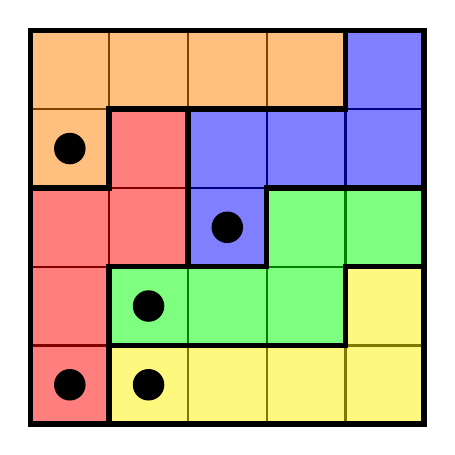
\begin{tikzpicture}
    \draw[thick] (0,0) grid (5,5);
    \draw[fill=red, fill opacity=0.5, line width=2] (0,0)--(0,3)--(1,3)--(1,4)--(2,4)--(2,2)--(1,2)--(1,0)--cycle;
    \draw[fill=orange, fill opacity=0.5, line width=2] (0,3)--(0,5)--(4,5)--(4,4)--(1,4)--(1,3)--cycle;
    \draw[fill=yellow, fill opacity=0.5, line width=2] (1,0)--(5,0)--(5,2)--(4,2)--(4,1)--(1,1)--cycle;
    \draw[fill=green, fill opacity=0.5, line width=2] (1,1)--(4,1)--(4,2)--(5,2)--(5,3)--(3,3)--(3,2)--(1,2)--cycle;
    \draw[fill=blue, fill opacity=0.5, line width=2] (2,2)--(3,2)--(3,3)--(5,3)--(5,5)--(4,5)--(4,4)--(2,4)--cycle;

    \fill
      (0.5, 0.5) circle (0.2)
      (1.5, 0.5) circle (0.2)
      (1.5, 1.5) circle (0.2)
      (0.5, 3.5) circle (0.2)
      (2.5, 2.5) circle (0.2)
    ;
  \end{tikzpicture}
  \caption{
    An example of a $5 \times 5$ grid with a unique solution.
  }
\end{figure}

\begin{question}
  How many $n \times n$ boards exist with a unique solution?
\end{question}

\begin{related}
  \item How many $n \times n$ boards exist with no solution? Multiple solutions?
  \item What board has the most solutions?
  \item What if this is counted up to dihedral action?
  \item What if this is done on an $n \times m$ board with $k$ marked cells where
  $k | nm$ and each region has $nm/k$ cells?
  \item What if the board is a torus? Triangular/hexagonal grid? Multiple dimensions?
  \item What if instead of marked cells there are marked regions? (e.g. two
  adjacent cells are both marked ``1'' and must be captured by the same region)
  \item What if cells must must be rectangular? Symmetric?
\end{related}


\begin{references}
  \item Problem 28
  \item \url{https://math.stackexchange.com/q/3072735/121988}
\end{references}

\end{document}
